\documentclass[fontsize=14pt]{extarticle}
\usepackage[a4paper, total={6in, 8in}]{geometry}
\usepackage{fontspec}
\usepackage{babel}
\usepackage{xcolor}
\usepackage{indentfirst}
\usepackage{graphicx}
\usepackage{datetime}
\usepackage{adjustbox}
\usepackage{makecell}
\graphicspath{ {./images/}}
\babelprovide[main, import]{thai}
\usepackage{hyperref}
\setmainfont[Path=fonts/,
 BoldFont={Sarabun-Bold.ttf}, 
 ItalicFont={Sarabun-Italic.ttf}, 
 BoldItalicFont={Sarabun-BoldItalic.ttf}, 
 ]{Sarabun-Regular.ttf}
\setmonofont[Path=fonts/]{Sarabun-Bold.ttf}
\geometry{margin=1in}
\ddmmyyyydate
\date{}

\title{\huge\textbf{Room Capacity Limiter}}
\author{Thanaphum Thepwan\\ Noppakorn Jiravaranun\\ Nopparuj Poonsubanan\\ Nanthicha Makjinda}
\begin{document}

\begin{center}
    \textbf{\Huge Room Capacity Limiter\\}
    \vspace*{\fill}
    {
        \LARGE
        \textbf{สมาชิก}\\~\\
        Thanaphum Thepwan 6330223021\\
        Noppakorn Jiravaranun 6330258021\\
        Nopparuj Poonsubanan 6330261921\\
        Nanthicha Makjinda 6330282021\\
        \vspace*{\fill}
        \textbf{เสนอ}\\~\\
        อ.ดร.พิชญะ สิทธิอมร\\
        \vspace*{\fill}
        รายงานนี้เป็นส่วนหนึ่งวิชา 2110366 Embedded System Laboratory\\
        ภาคการศึกษาปลาย ปีการศึกษา 2564
    }
\end{center}
\pagebreak
\tableofcontents
\pagebreak
\section{Description}
อุปกรณ์นี้เป็นอุปกรณ์สำหรับจำกัดจำนวนนิสิต หรือคนภายในห้อง ซึ่งต้องมีการแตะบัตรนิสิต หรือบัตร RFID ก่อนเข้าสถานที่ต่างๆ
โดยจะบอกว่าตอนนี้มีคนอยู่ในห้องนั้นๆ กี่คนซึ่งเข้ากับสถานการณ์ระบาดของไวรัส COVID-19
ซึ่งในปัจจุบันมีการรณรงค์การ Social Distancing และ ลดการสัมผัสซึ่งอุปกรณ์ที่ออกแบบสามารถตอบสนองการใช้งานในส่วนนี้ได้เป็นอย่างดีโดยสามารถลดการ
สัมผัสระหว่างบุคคล และสามารถทำให้การตรวจชื่อนิสิต หรือคนที่อยู่ในห้องได้สะดวกขึ้น และยังประยุกต์หลักการของ IoT
เข้ามาเพื่อช่วยให้สามารถแสดงผลการทํางาน ของอุปกรณ์ได้แบบ Real time
\section{Device}
อุปกรณ์ที่ใช้ประกอบด้วย\\
\begin{enumerate}
    \item STM32 NUCLEO F411-RE
    \item ESP8266
    \item RFID-RC522
    \item LCD Screen (LCD1602)
\end{enumerate}
\section{Website}
\url{https://embedded-project.vercel.app}
\section{Source Code}
Source Code และเอกสารเกี่ยวกับ Project สามารถเข้าถึงได้ที่ \url{https://github.com/noppakorn/embedded-project}
\pagebreak
\section{Roles and Responsibility}
\subsection{Team Management}
By: Thanaphum Thepwan\\
\subsubsection{Responsibility}
\begin{itemize}
    \item เสนอหัวข้อ Project ในการทำงาน
    \item ประสานงานกับทุกฝ่ายในกลุ่มในการกำหนดวันในการมาทำงานร่วมกัน การแบ่งงานในแต่ละส่วน
    \item จัดทำส่วนของการ Presentation
    \item ดูภาพรวมของ Project ให้เป็นไปตามเป้าหมาย
\end{itemize}
จากโจทย์ในการทำงานได้มาว่า Contactless Society ซึ่งจากการเป็น Team Management ซึ่งหัวข้อที่ได้เสนอไปก็คือ ทำระบบจำกัดจำนวนคนในห้องใช้ระบบ Checkin โดยใช้บัตรนิสิต หรือบัตร RFID ซึ่งเมื่อตกลงกันในกลุ่มแล้ว ได้\\กำหนดช่องทางการสื่อสารหลักเป็น Discord และได้แบ่งงานให้แต่ละคนดังนี้
\begin{enumerate}
    \item Nanthicha: System Architecture\\ (จัดหา sensor ต่างๆที่ต้องใช้ ออกแบบระบบว่าแต่ละอุปกรณ์เชื่อมต่อกันได้อย่างไร)
    \item Noppakorn: Embedded System Development \\ (การโปรแกรมลง Board)
    \item Nopparuj: รับผิดชอบในส่วนของ UI/UX Designer and Development\\ (ออกแบบพัฒนาเว็บไซต์)
\end{enumerate}
\subsubsection{Plan}
\begin{center}
    \begin{adjustbox}{width=\textwidth}
        \begin{tabular}{ | c | c |  }
            \hline
            งาน & วันที่ดำเนินงาน \\
            \hline
            \hline
            กำหนดหัวข้อโปรเจกต์จากโจทย์ที่ได้รับ & \formatdate{12}{04}{2022} \\
            \hline
            เริ่มจัดทำ frontend & \formatdate{13}{04}{2022} \\
            \hline
            ทำให้ส่วนของ frontend สามารถ fetch ข้อมูลจาก firebase ได้ & \formatdate{18}{04}{2022} \\
            \hline
            นำเสนอหัวข้อโปรเจกต์ให้อาจารย์อนุมัติ และได้กำหนดอุปกรณ์ที่ต้องใช้ & \formatdate{20}{04}{2022} \\                 
            \hline
            \makecell{ทำงานร่วมกันครั้งแรก รับ ESP8266, RFID-RC522\\และโปรแกรมทำให้ ESP8266 สามารถเชื่อม Internet ได้} & \formatdate{27}{04}{2022} \\
            \hline
            เชื่อมต่อกับเซนเซอร์ RFID-RC522 ให้สามารถอ่านบัตรได้ & \formatdate{03}{05}{2022} ถึง \formatdate{20}{05}{2022} \\
            \hline
            ทำให้ข้อมูลที่อ่านได้จาก RFID-RC522 สามารถส่งขึ้นไปที่ Cloud ได้ & \formatdate{23}{05}{2022} \\
            \hline
            \makecell{ทำให้ Cloud Response data กลับมาที่ ESP8266 \\เพื่อที่จะนำข้อมูลไปแสดงบนหน้าจอ LCD } & \formatdate{25}{05}{2022} \\
            \hline
            เชื่อมต่อจอ LCD Screen เพื่อให้สามารถแสดงข้อมูลได้จาก Cloud & \formatdate{27}{05}{2022} \\
            \hline
            จัดทำ Presentation และ Report & \formatdate{31}{05}{2022}\\
            \hline
        \end{tabular}
    \end{adjustbox}
\end{center}
\pagebreak
\subsection{System Architecture}
By: Nanthicha Makjinda \\
\subsubsection{Responsibility}
\begin{enumerate}
    \item Hardware Design: กำหนด sensor ที่ต้องใช้ในระบบทั้งหมด
    \item Database Design: ออกแบบโครงสร้าง Database
    \item API Design: ออกแบบโครงสร้าง API เพื่อการติดต่อของ ESP8266
\end{enumerate}
\subsubsection{Hardware Design}
ระบบจะต้องมีรายละเอียดและสามารถทำงานได้ดังนี้
\begin{itemize}
    \item สามารถแตะบัตรและอ่านข้อมูล id ของบัตรได้โดยใช้ sensor RFID Reader
    \item สามารถแสดงผลการ check in ให้ผู้ใช้งานทราบเมื่อมีการแตะบัตร โดยแสดงผลผ่าน LCD Screen
    \item สามารถใช้ internet ในการติดต่อกับ API เพื่อเพิ่มนักเรียนเข้าไปในห้องหรือเรียกดูข้อมูลนักเรียนได้โดยใช้ NodeMCU
\end{itemize}
\subsubsection{Database Design}
โครงสร้าง Database (Firestore Database) แบ่งออกเป็น 3 collections ได้แก่
  \begin{itemize}
      \item room
            เก็บข้อมูลนักเรียนที่ทำการแตะบัตร check in เข้าห้อง โดยในแต่ละ document ใน collection เก็บข้อมูล รหัสนิสิต ชื่อ-นามสกุล และ เวลาที่ทำการ check in
      \item room-detail
            เก็บข้อมูล capacity ของห้อง
      \item students-name
            เก็บข้อมูลนักเรียน ชื่อ-นามสกุล รหัสนิสิต โดยอ้างอิงกับบัตรนิสิตที่จะใช้ในการแตะ check in เข้าห้อง
  \end{itemize}
\subsubsection{API Design}
\par การใช้งาน Embedded System กับ Firebase Firestore Database นั้นมีขั้นตอนการใช้งานที่ยุ่งยาก อีกทั้งยังต้องมี Boilerplate Code จำนวนมากในการใช้งาน และ Library ยังมี Feature  น้อยกว่า Library ใน JS ecosystem เป็นอย่างมาก จึงมีการ Design API เพื่อทำให้การ Development ของ Embedded System สะดวกขึ้นอีกทั้งยังเป็นการลดภาระของ Embedded System ทำให้ระบบมีประสิทธิภาพและความยืดหยุ่นมากขึ้น
\par โดย Frontend มีการใช้งาน Next.js ซึ่งเป็น Frontend Web Developement Framework ที่มี Feature Next API ทำให้การสร้าง API สามารถทำได้ง่าย และสามารถนำไป Host ที่ Vercel ในที่เดียวกับ Website ได้เลยโดยไม่ทีค่าใช้จ่าย
\par API นั้นเขียนโดยภาษา TypeScript โดยเป็น REST API ซึ่งทำการ handle POST Request โดย Embedded System นั่นคือ ESP8266 นั้นสามารถส่ง POST Request มายัง API ที่ \url{https://embedded-project.vercel.app/api/user} โดยใน request ส่งข้อมูลในรูปแบบ JSON โดยประกอบด้วย field card id โดย เป็น string hexadeciamal 10 หลัก จากนั้น API จะทำการตรวจสอบจาก database ว่ามีนิสิตคนนี้ในระบบหรือไม่ และทำการ Check in และ Check out ออกจากห้องเรียนนั้นๆ อีกทั้งยังมีการเช็คจำนวนนิสิตในห้องเรียน แล้วจึงตอบเป็น status ไปยัง ESP8266 เพื่อทำการประมวลผลและทำการแสดงผลต่อไป\\
Source Code ของ API อยู่ที่ \url{https://github.com/noppakorn/embedded-project/blob/main/frontend/pages/api/user.ts}
\pagebreak
\subsection{Embedded System Development}
By: Noppakorn Jiravaranun\\
\subsubsection{Responsibility}
\begin{itemize}
    \item การเชื่อมต่อระหว่าง Sensor และ Hardware
    \item การโปรแกรม STM32
    \item การโปรแกรม ESP8266
    \item การเชื่อมต่อของ ESP8266 กับ API
\end{itemize}
\subsubsection{Hardware Connectivity}
Hardware ทั้งหมดเชื่อต่อกันโดยมี STM32 NUCLEO F411-RE เป็นศูนย์กลาง โดยมีการเชื่อมต่อกันดังน้ี
\begin{enumerate}
    \item NodeMCU ESP8266 เชื่อมต่อกับ STM32 โดย I2C โดย ESP8266 เป็น master
    \item RFID Reader RC522 เชื่อมต่อกับ STM32 โดย SPI
    \item LCD Screen (LCD1602) เชื่อมต่อกับ STM32 โดย I2C
\end{enumerate}
\begin{center}
    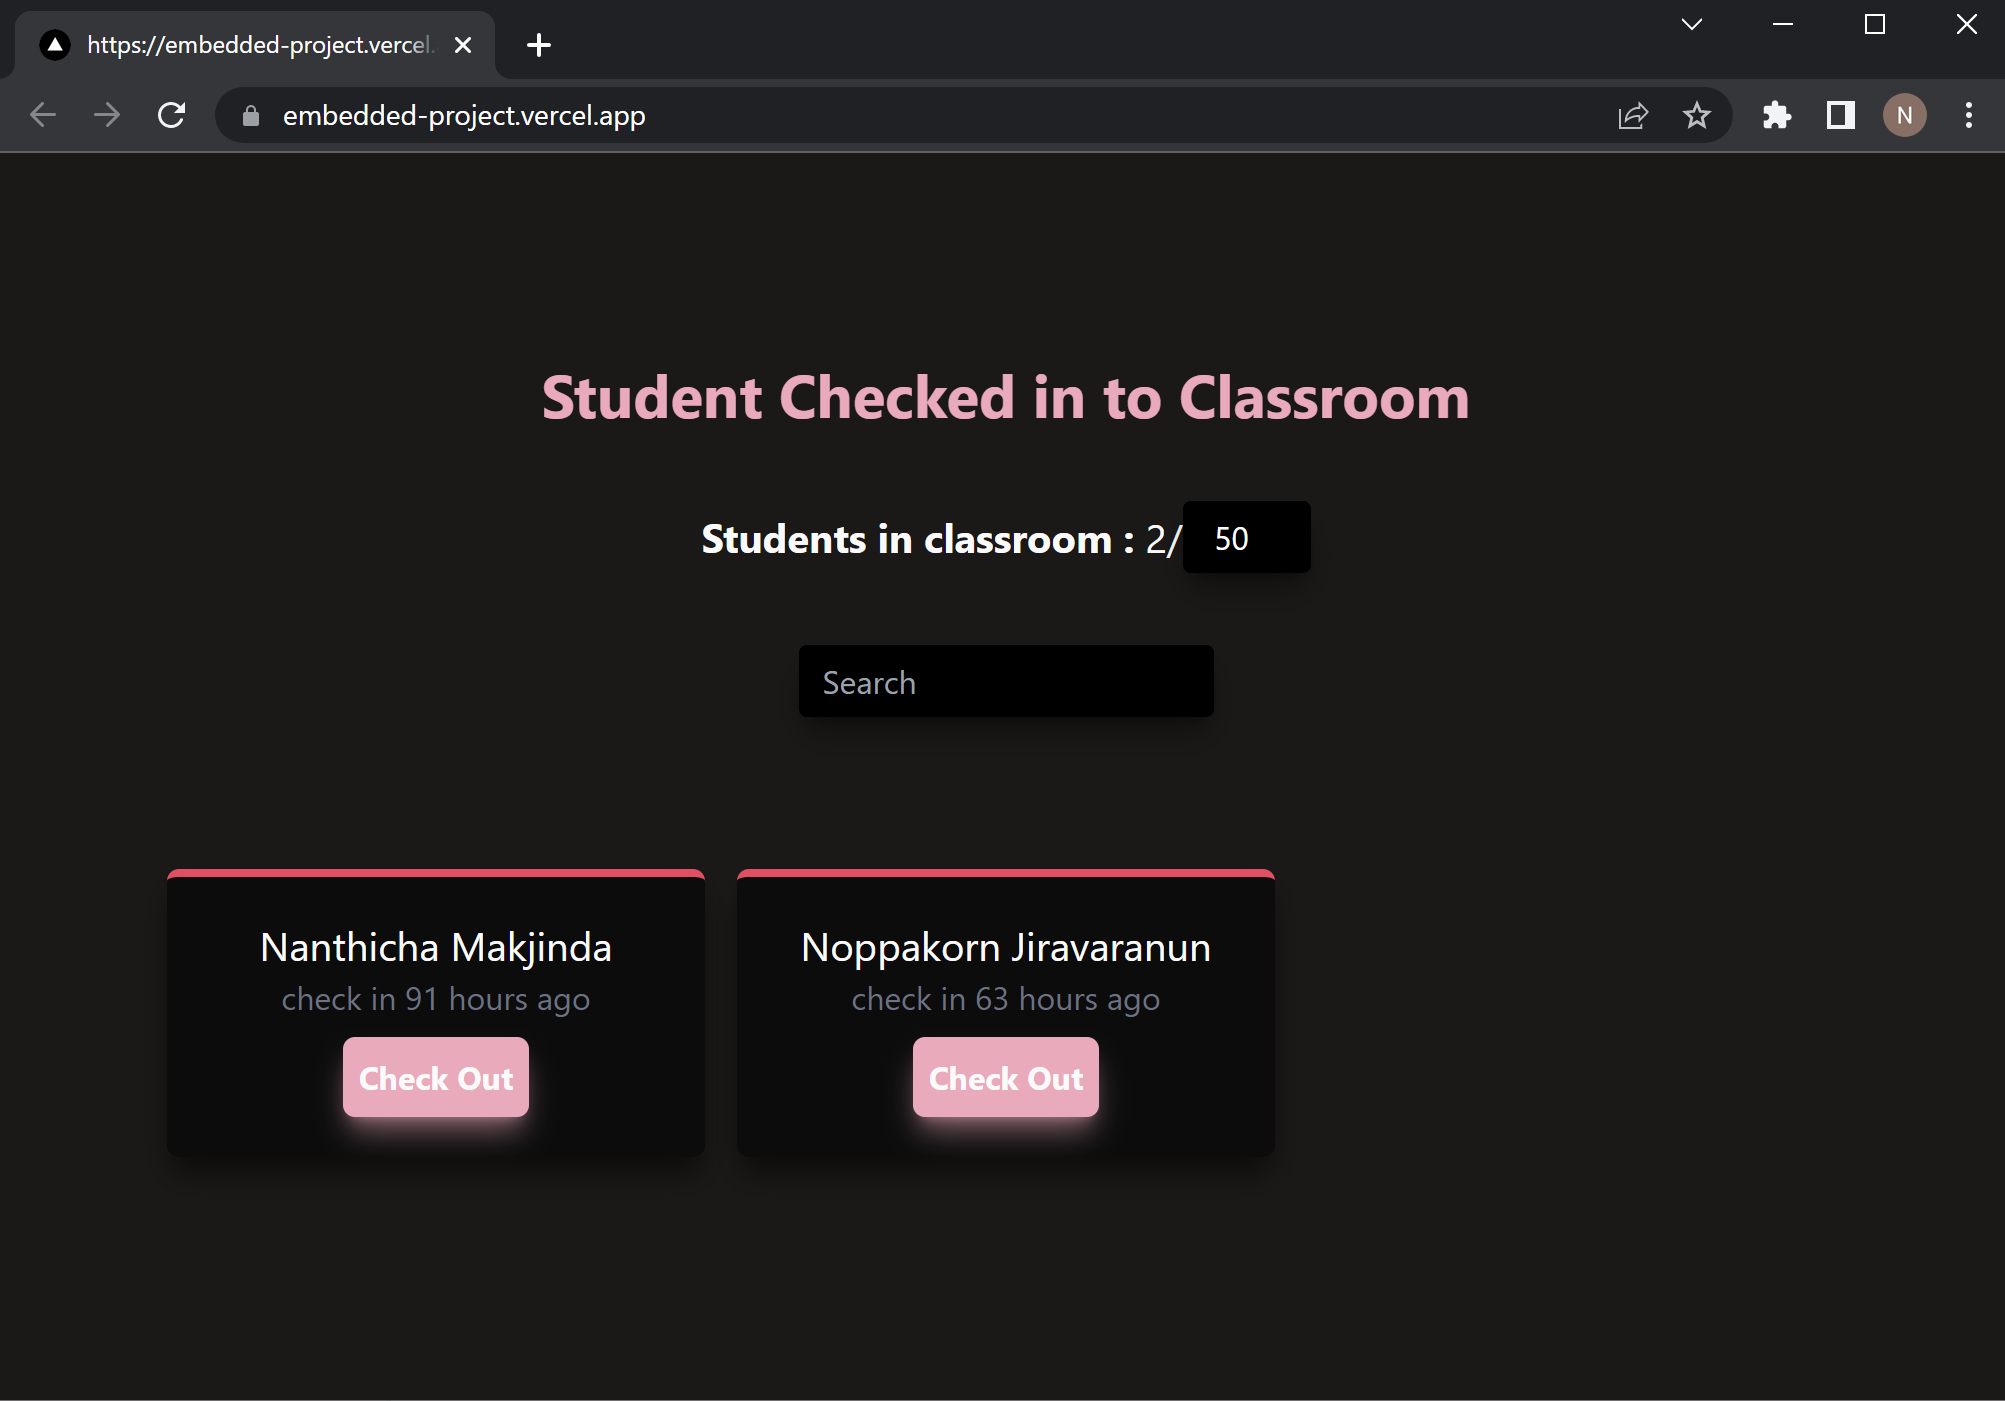
\includegraphics[width=\textwidth]{Web.png}
\end{center}
\pagebreak
\subsubsection{หน้าที่ของ Hardware}
\begin{itemize}
    \item STM32 NUCLEO F411-RE มีหน้าที่เป็นศูนย์กลางการเชื่อมต่อระหว่าง Hardware ต่างๆ และประมวลผลที่ได้รับจาก NodeMCU
    \item NodeMCU ESP8266 มีหน้าที่ติดต่อไปยัง API ที่ Host บน Vercel  โดยทำการ ส่ง GET และ POST Request ไปยัง \\ \url{https://embedded-project.vercel.app/api/user}  โดยส่งเป็นรหัสของบัตรนิสิต และจะได้ Response เป็นผลของการ Check In หรือ Check Out และทำการประมวลผลในขั้นต้นเพื่อให้ง่ายต่อการน้ำข้อมูลไปใช้บน STM32
    \item RFID Reader RC522 มีหน้าที่อ่านบัตรนิสิตเพื่อส่งข้อมูลให้ STM32
    \item LCD Screen (LCD1602) มีหน้าที่แสดงผลการ Check In ให้ผู้ใช้ทราบ
\end{itemize}
\subsubsection{การทำงานของ Embedded System}
\begin{enumerate}
    \item STM32 คอยตรวจสอบบัตร  ผ่าน RFID Reader RC522 เมื่อพบบัตรจึงส่ง Card ID ไปยัง ESP8266 ผ่าน I2C
    \item เมื่อ ESP8266 ได้รับข้อมูลผ่าน I2C จึงส่งข้อมูลไปยัง api ที่ Vercel เมื่อได้รับข้อมูลกลับมา จึงส่งข้อมูลกลับไปยัง STM32
    \item เมื่อ STM32 ได้รับข้อมูลกลับมาจึงประมวลผลที่ได้รับและแสดงผลผ่าน LCD Screen เพื่อให้ User ทราบ
    \item เมื่อจบกระบวนการจึงกลับไปเริ่มในขั้นตอนแรก
\end{enumerate}
\pagebreak
\subsection{UI/UX Designer and Development}
By: Nopparuj Poonsubanan
\subsubsection{Responsibility}
\begin{enumerate}
    \item UI/UX Design: กำหนด Feature ของเว็บและการใช้งานของ user ให้มีประสิทธิภาพ และใช้งานง่าย อีกทั้งยังมีการ Design ความสวยงามของ UI
    \item Web Development นำ Design ที่กำหนดไว้ในขั้นตอน UI/UX Design มาทำเป็นเว็บไซต์
\end{enumerate}
\subsubsection{UI Design}
    แบ่งส่วนแสดงผลออกเป็น 3 ส่วน ได้แก่
    \begin{enumerate}
        \item ส่วนแสดงข้อมูลจำนวนนักเรียนภายในห้องและแก้ไข capacity ของห้อง
        \item ส่วน search box ใช้ในการค้นหานักเรียนในห้อง
        \item ส่วนที่แสดงข้อมูลรายละเอียดของนักเรียนแต่ละคนที่ check in เข้าห้อง โดยจะมีการแสดงเวลาที่นักเรียนอยู่ในห้องและมีปุ่มสำหรับการ check out
    \end{enumerate}
\subsubsection{Web Development}
\par Web Development นั้นได้ปฎิบัติงานโดยนำ Frontend Design ที่กำหนดไว้ในขั้นตอนการ Design UX/UI มาสร้างเป็น Single Page Application
\par ในงานนี้เลือกใช้ Next.js เป็น Frontend Web Development Framework เนื่องจากง่ายในการใช้งาน อีกทั้งยังมี Next API ที่ built-in ใน frontend อีกทั้งยังสามารถ Deploy ไปยัง Vercel ได้อย่างง่ายดาย
\par เว็บไซต์ใช้การดึงข้อมูลจาก Firebase มาแสดงผล การแก้ไขข้อมูต่างๆ ใน Firebase ไม่ว่าการแก้ไขจาก Embedded System หรือการแก้ไขจากหน้าเว็บจะได้รับการอัพเดตโดยทันทีโดยไม่ต้องมี Interaction จาก user
\pagebreak

\end{document}